\documentclass[11pt]{article}

\usepackage[a4paper, margin=1in]{geometry}
\usepackage[T1]{fontenc}
\usepackage{helvet}

\usepackage{tabularx}
\usepackage{ragged2e}

\usepackage{float}
\usepackage{csquotes}
\usepackage{amsmath}
\usepackage{amsfonts}
\usepackage{latexsym}
\usepackage{graphicx}

\usepackage[shortlabels]{enumitem}

\usepackage[hidelinks]{hyperref}

\setlength{\parindent}{0pt}
\setlength{\parskip}{1em}
\renewcommand{\familydefault}{\sfdefault}

\renewcommand{\thesubsection}{\thesection.\alph{subsection}}

\title{CS3101 - Databases Exam}
\author{200007413}
\date{22 Apr 2023}

\begin{document}

    \maketitle

    \section{TODO}
    
    \subsection{}

    For this scenario, I assumed that the ISBN are unique across all volumes,
    editions, and versions.

    \begin{figure}[H]
        \centering
        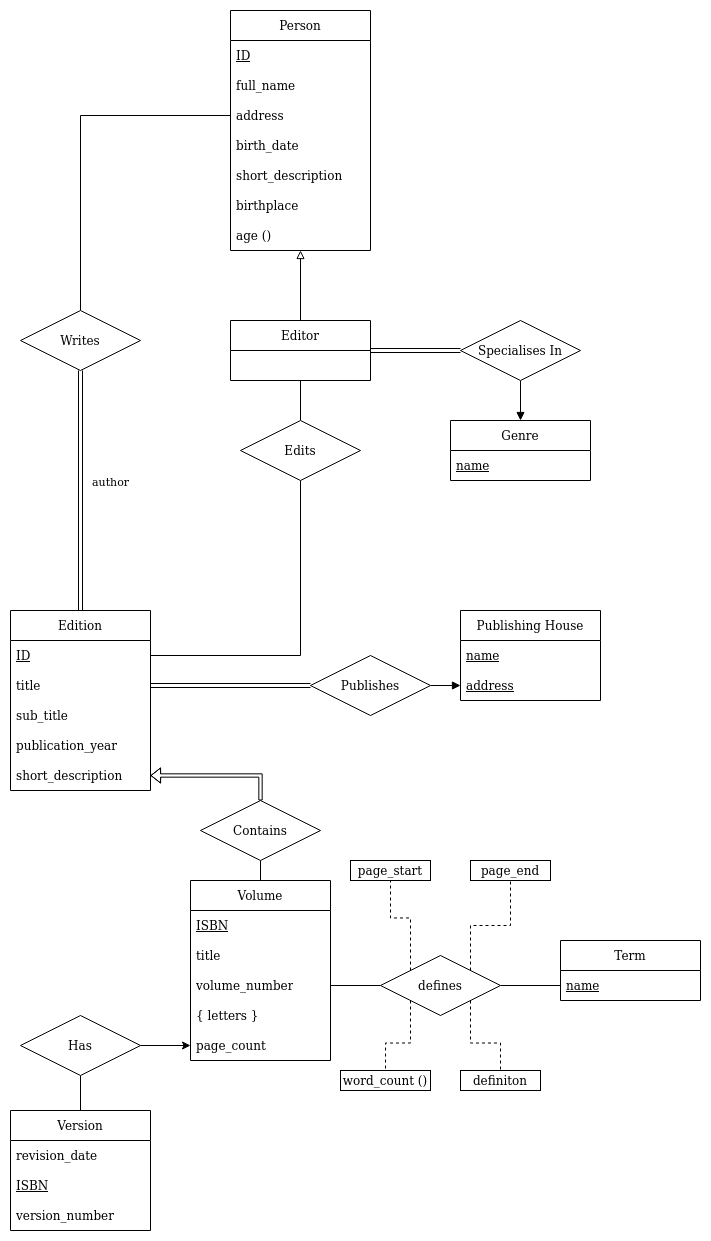
\includegraphics[width=0.8\linewidth]{Q1.png}
    \end{figure}

    \subsection{}

    person($\underline{\text{id}}$, full\_name, address, birth\_date, short\_description,
    birthplace)

    editor\_specialty($\underline{\text{person\_id*}}, \underline{\text{genre\_name}}$)

    writes($\underline{\text{person\_id*}}, \underline{\text{edition\_id*}}$)

    edits($\underline{\text{person\_id*}}, \underline{\text{edition\_id*}}$)

    edition($\underline{\text{id}}$, title, sub\_title, publication\_year,
    short\_description)

    publishing\_house($\underline{\text{name}, \text{address}}$)

    edition\_publisher($\underline{\text{publisher\_name}, \text{address}}$)

    \subsection{}

    \subsubsection{}

    SELECT id, publication\_year FROM edition

    \subsubsection{}

    SELECT e.id, COUNT(v.ISBN) AS count FROM edition as e LEFT JOIN volume as v ON
    v.edition\_id = e.id WHERE e.publication\_year < 1850
    GROUP BY e.edition\_id

    \subsubsection{}

    SELECT start\_page, end\_page FROM term\_definition AS td LEFT JOIN volume AS v ON td.volume\_ISBN = v.ISBN WHERE td.name = "abacus" AND exists (SELECT * FROM edititon as e WHERE e.id = v.edition\_id AND e.id = 1)

    \section{}

    \subsection{}

    \subsubsection{}

    \begin{tabular}{r l}
        student = \{  & id $\rightarrow$ name \\
        \}\\
        tutors = \{ & tutor\_id $\rightarrow$ tutor\_email \\
        \}\\
        practical\_grade = \{ & student\_id,module\_id,practical\_number $\rightarrow$ grade \\
        \}\\
    \end{tabular}

    \subsubsection{}

    At the given exact moment, there would be a functional dependency between
    module\_id and practical\_number, as each value of module\_id refers to a
    unique practical\_number. 

    However, this functional dependency will not exist once a second practical
    for a module is added, as then one module is not guaranteed to reference a
    unique practical\_id.

    \subsection{}

    \subsubsection{}

    Yes, the \textit{tutors} relation is in first normal form, as all it's
    attributes are atomic. Each tuple refers to a single student using
    student\_id, and refers to a single staff member using tutor\_id, with a
    single email.
    
    \subsubsection{}

    Yes, because \textit{tutors} is in first normal form, and each of the
    attributes are either candidate keys or full functionally dependent on a
    candidate key.

    Both tutor\_id and student\_id are required to uniquely identify the
    relationship, and so are candidate keys, and then tutor\_email is
    functionally dependent on the tutor\_id.

    \subsubsection{}

    Under the assumption that tutors do not have more than one email address,
    \textit{tutors} is not in third normal form. 

    Whilst it is in second normal form, and tutor\_id and student\_id are part
    of the super-key, tutor\_id itself is not a superkey, and there is a
    functional dependency from tutor\_id to the non-candidate-key attribute
    tutor\_email. Additionally, tutor\_email-tutor\_id = tutor\_email, which is
    itself not in a candiate key.

    \subsubsection{}

    This is not in Boyce-Codd normal form (BCNF) as it is not in third-normal
    form.

    The condition for BCNF is the same as 3NF in that every functional
    dependency $\alpha \rightarrow \beta$ must either be trivial or be
    dependent on a superkey, with the added restriction that $\beta - \alpha$
    being in a candidate key is not sufficient. As the tutor\_id $\rightarrow$
    tutor\_email already doesn't meet the less strict 3NF conditions, it does
    not meet BCNF.

    \subsection{}

    Artificial primary keys are those which do not relate to any real data, but
    are added to ensure that there is a unique identifier for each entry,
    instead of relying upon the three natural candidate keys to uniquely
    identify each tuple.

    The advantages to using the artificial ID value is that you can create
    queries using just that identifier, instead of requiring that someone know
    the module\_id, student\_id, and practical\_number. Practically, this could
    allow students to access their practical grades just with the
    practical\_grade ID.

    The downside to using the ID attribute is it will add redundant
    information, and prevent the schema from being in Boyce-Codd normal form.
    This is because each entry is already unqiuely identified using the three
    candidate keys, and so the ID is functionally dependent on these and
    visa-versa.

    This redundancy would add additional space requirements for storing the
    table, as a new not-strictly required column is added to each tuple.

    Another risk from artificial keys is with the chance for duplicate entries.
    If ID is set as the sole unique superkey, then more than one entry could
    point to the same "useful" data, but just with a new ID, practically adding
    duplicate data. Without artificial keys, only unique combinations of
    student\_id,module\_id, and practical\_number can be added.

    \subsection{TODO}


\section{}

\subsection{}

A \textit{mediumblob}/\textit{longblob} type may be appropriate for \textit{user.picture} for
storing the raw picture data itself. This would be a large data type, and would
store the picture in the database.

Another appropriate type could be a \textit{varchar}, which would contain the
URL to that user's picture. 

The benefit of a blob data type is that no additional calls need to be made to
retrieve the users profile picture, as the call itself returns it's raw data.

However, this means the database will be much larger than having a varchar
containing a url.

Another advantage of the varchar URL method is the image can
be stored at the URL as an image file. Storing as a blob ignores the file tyoe,
meaning the program accessing the data must interpret the image properly.
Storing the image as a file can prevent the need to interpret raw data in this
way.

\subsection{}

\subsubsection{}

$$\Pi_{\text{username}}(\sigma_{\text{rating} > 1800}(\text{user}))$$

\subsubsection{}

$\Pi_{\text{p1\_username}}(\text{game} \Join \sigma_{\text{name} = \text{"Sammy Jacobs Cup"}}(\text{tournament}))$

\subsection{}

SELECT UNIQUE p1\_username FROM game WHERE EXISTS (SELECT tournament\_id FROM tournament
WHERE tournament\_id = id AND tournament.name = "Sammy Jacobs Cup")

\subsection{}

\subsubsection{}

manutdlover \\

joker77,manudlover,tobym \\

alan34,alexr,bigbob joker77,kingkhalid,md216 mudlover,ohio\_alice,pkg113 tobym  \\

\subsubsection{}

Increasing the value of N would allow for more items to be added before the
tree needs to be reorganized. 

An issue with this is that the graph would become more uneven, thus reducing
the efficiency when searching.

\subsubsection{}

The advantage of a hash index is that exact match queries are much faster. An
example of a query which would run faster for a hash index would be:

SELECT * FROM user WHERE username = "bob"

Queries which have non-exact matching criteria would be faster for B+ indexes.
For example:

SELECT * FROM user WHERE username LIKE "bo\%son"

\end{document}
